\section[The Gravity Framework in international Trade]{The Gravity Framework in international Trade$^{\text{ AA, JE}}$}
\label{sec:Gravity_Framework}

The gravity model of trade has its roots in Newtonian physics, where the force of gravity between two objects is directly proportional to their masses and inversely proportional to the square of the distance between them. Similarly, the gravity equation in international trade posits that the volume of trade between two countries is directly proportional to their economic size, usually measured by GDP, and inversely proportional to the distance between them. \textcite{tinbergen1962shaping} is often cited as the first to apply this concept to international trade, proposing that larger economies trade more with each other and that trade diminishes with increasing distance.

\textcite{Anderson2003} introduced significant refinements to the gravity model by addressing the issue of \textit{multilateral resistance}. They argued that trade flows between two countries depend not only on their bilateral distance but also on their relative distances to all other trading partners. This adjustment accounts for the fact that a country’s trade is influenced by its position in the global trade network.

Due to the high amount of textbooks and scientific papers that incorporated the gravity framework over the last decades, formal notations differ substantially. In this section, we present the linkages of the gravity framework to international trade theory and discuss the main empirical estimation strategies to provide the reader with a basic understanding of challenges when it comes to combining theory with data. Therefore, we utilize the notation style of \textcite[p. 17]{yotov2016advanced}, who provide an advanced guide for researchers who aim to construct a gravity analysis. To capture both the original idea of \textcite{tinbergen1962shaping} and the extension of \textcite{Anderson2003}, they denote the \textit{structural gravity model} as shown in equation \ref{eq:Structural_Model_NF}: \begin{equation}
    \label{eq:Structural_Model_NF}
    X_{ij} = \Tilde{G} \frac{Y_i E_j }{T_{ij}^{\Theta}}
\end{equation} In this notation $X_{ij}$ represents exports from country i and j, $\Tilde{G}$ is the inverse of the total world production ($\Tilde{G} \equiv 1/Y$), $Y_i$ is country $i$'s domestic production, $E_i$ is country $j$'s aggregate expenditure and $T_{ij}^{\Theta}$ are the total trade costs between countries $i$ and $j$. Finally, $T_{ij}^{\Theta} \equiv \left( t_{ij}/(\Pi_i P_j) \right)^{\sigma - 1}$ is a term that includes all costs of trade, where $t_{ij}$\footnote{Finding fitting proxies for $t_{ij}$ is an ongoing challenge in the empirical literature and will be discussed in depth in section \ref{sec:Determinants_of_Trade}.} are bilateral trade costs between economies, $\Pi_i$ is a structural term to capture the idea of multilateral resistance by \textcite{Anderson2003} and can be interpreted as market access abilities of an exporting country $i$ (\textit{outward} multilateral resistance), while $P_j$ captures an importing country's market access ability as \textit{inward} multilateral resistance (\cite[p. 16]{yotov2016advanced}).\footnote{\textcite[pp. 13-17]{yotov2016advanced} also provide a formal demand side derivation of the structural gravity model, while a supply side derivation is shown in their appendix.} Considering a model with $t$ periods, to obtain an easily estimable structural gravity equation, expression \ref{eq:Structural_Model_NF} can be log-linearized. \begin{equation}
    \label{eq:Structural_Model_LIN}
    \ln{X_{ij,t}} = \ln{E_{j,t}} + \ln{Y_{i,t}} - \ln{Y_t} + (1-\sigma) \ln{t_{ij,t}} - (1-\sigma) \ln{P_{j,t}} - (1-\sigma) \ln{\Pi_{i,t}} + \epsilon_{ij,t}
\end{equation} Equation \ref{eq:Structural_Model_LIN} than represents a theory founded model that can be estimated using econometric methods. Note that the error term $\epsilon_{ij,t}$ is introduced to capture noise in the data (\cite[p. 17]{yotov2016advanced}). In what follows, a brief overview of how equations \ref{eq:Structural_Model_NF} and \ref{eq:Structural_Model_LIN} are linked to well developed international trade theories (section \ref{subsec:theoretic_foundations}) is given. Furthermore, challenges when it comes to estimating equation \ref{eq:Structural_Model_LIN} are reviewed (section \ref{subsec:estimation_tools}) in order to generate a basic understanding of the discipline. This enables the reader to better focus on the reasoning in following chapters.











\subsection[Theoretic Foundations]{Theoretic Foundations$^{\text{ AA}}$}
\label{subsec:theoretic_foundations}

Trade has always been acknowledged as a factor, in promoting unity and fostering peace among nations. The belief that interconnected markets lead to benefits and stability has historical roots, especially evident in the relationship between the U.S. And Europe, where trade has often played a role in maintaining peace and strengthening economic connections. This viewpoint holds relevance today given the increasing tensions and the volatile nature of the global economy. Therefore analyzing trade patterns and understanding what drives trade have become tasks for researchers seeking to shed light on how trade can contribute to stability and prosperity.

The gravity model stands out as a tool for studying trade dynamics. Similar to its namesake concept in physics this model suggests that the volume of trade between two countries is directly related to their sizes while being inversely proportional to the distance separating them. This model has demonstrated power in understanding trade patterns and has been widely utilized to identify irregularities and explore the factors influencing trade volumes. Renowned economist Paul Krugman emphasizes the significance of gravity analysis in uncovering these irregularities and examining socio linguistic and geographic factors that affect international trade .

Inspired by Newtons law of gravity the gravity model of trade has long been a principle, in economics.
This theory suggests that the amount of trade, between two countries is directly linked to their strength usually measured by GDP and inversely related to the distance separating them (\cite{tinbergen1962shaping}). While using gravity equations has shed light on the patterns and factors influencing goods trade the changing global economy requires an evaluation of their relevance to services trade.

Since the 1990s services trade has shown growth rates compared to aspects of international trade (Breinlich et al. as cited in WTO). Services have become a part of trade covering various activities like financial services, tourism, information technology and professional services. Unlike goods trade services involve features such as intangibility, diversity and the need for interactions between producers and consumers. This often blurs regulatory boundaries. These differences lead to questions; do gravity equations work well for goods and services trade? Are the factors influencing and hindering trade the same, in both sectors?

This article explores these questions by offering an examination of gravity equations concerning goods and services trade.
The gravity model is thoroughly explored in this study analyzing research findings and emphasizing the varying impacts of distance economic size and other variables, on the trade of goods versus services. \textcite{Anderson2003} refined the model to address resistance factors for understanding trade dynamics in both sectors. \textcite{Kimura2006} underscored the need to consider service characteristics when using gravity equations as traditional models may not fully capture service trade dynamics.

Moreover studies by \textcite{NBERw12516} and \textcite{EGGER2011263} have shown that while gravity equations can apply to both goods and services their sensitivity to factors like distance and economic integration differs significantly between the two. \textcite{Bergstrand_1985} highlighted the roots of the gravity equation suggesting that distinct factors drive goods, versus services trade.

This analysis aims to determine whether a unified model can effectively capture the complexities of both goods and services trade or if adjustments are needed to accommodate the nature of services.
This study not enhances our comprehension of trade but also offers valuable perspectives for decision makers seeking to promote economic growth by easing trade restrictions.



% 6.Krugman, P. (2019). International Economics: Theory and Policy. [Page 41].


% 8.Yotov, Y. V., Piermartini, R., Monteiro, J. A., \& Larch, M. (2016). An Advanced Guide to Trade Policy Analysis: The Structural Gravity Model. [Page 17].



% Here comes the section about theoretic foundations:



\begin{figure}[htbp]
    \centering
    \caption[Gravity model's strong theoretical foundations]{Gravity model's strong theoretical foundations}
    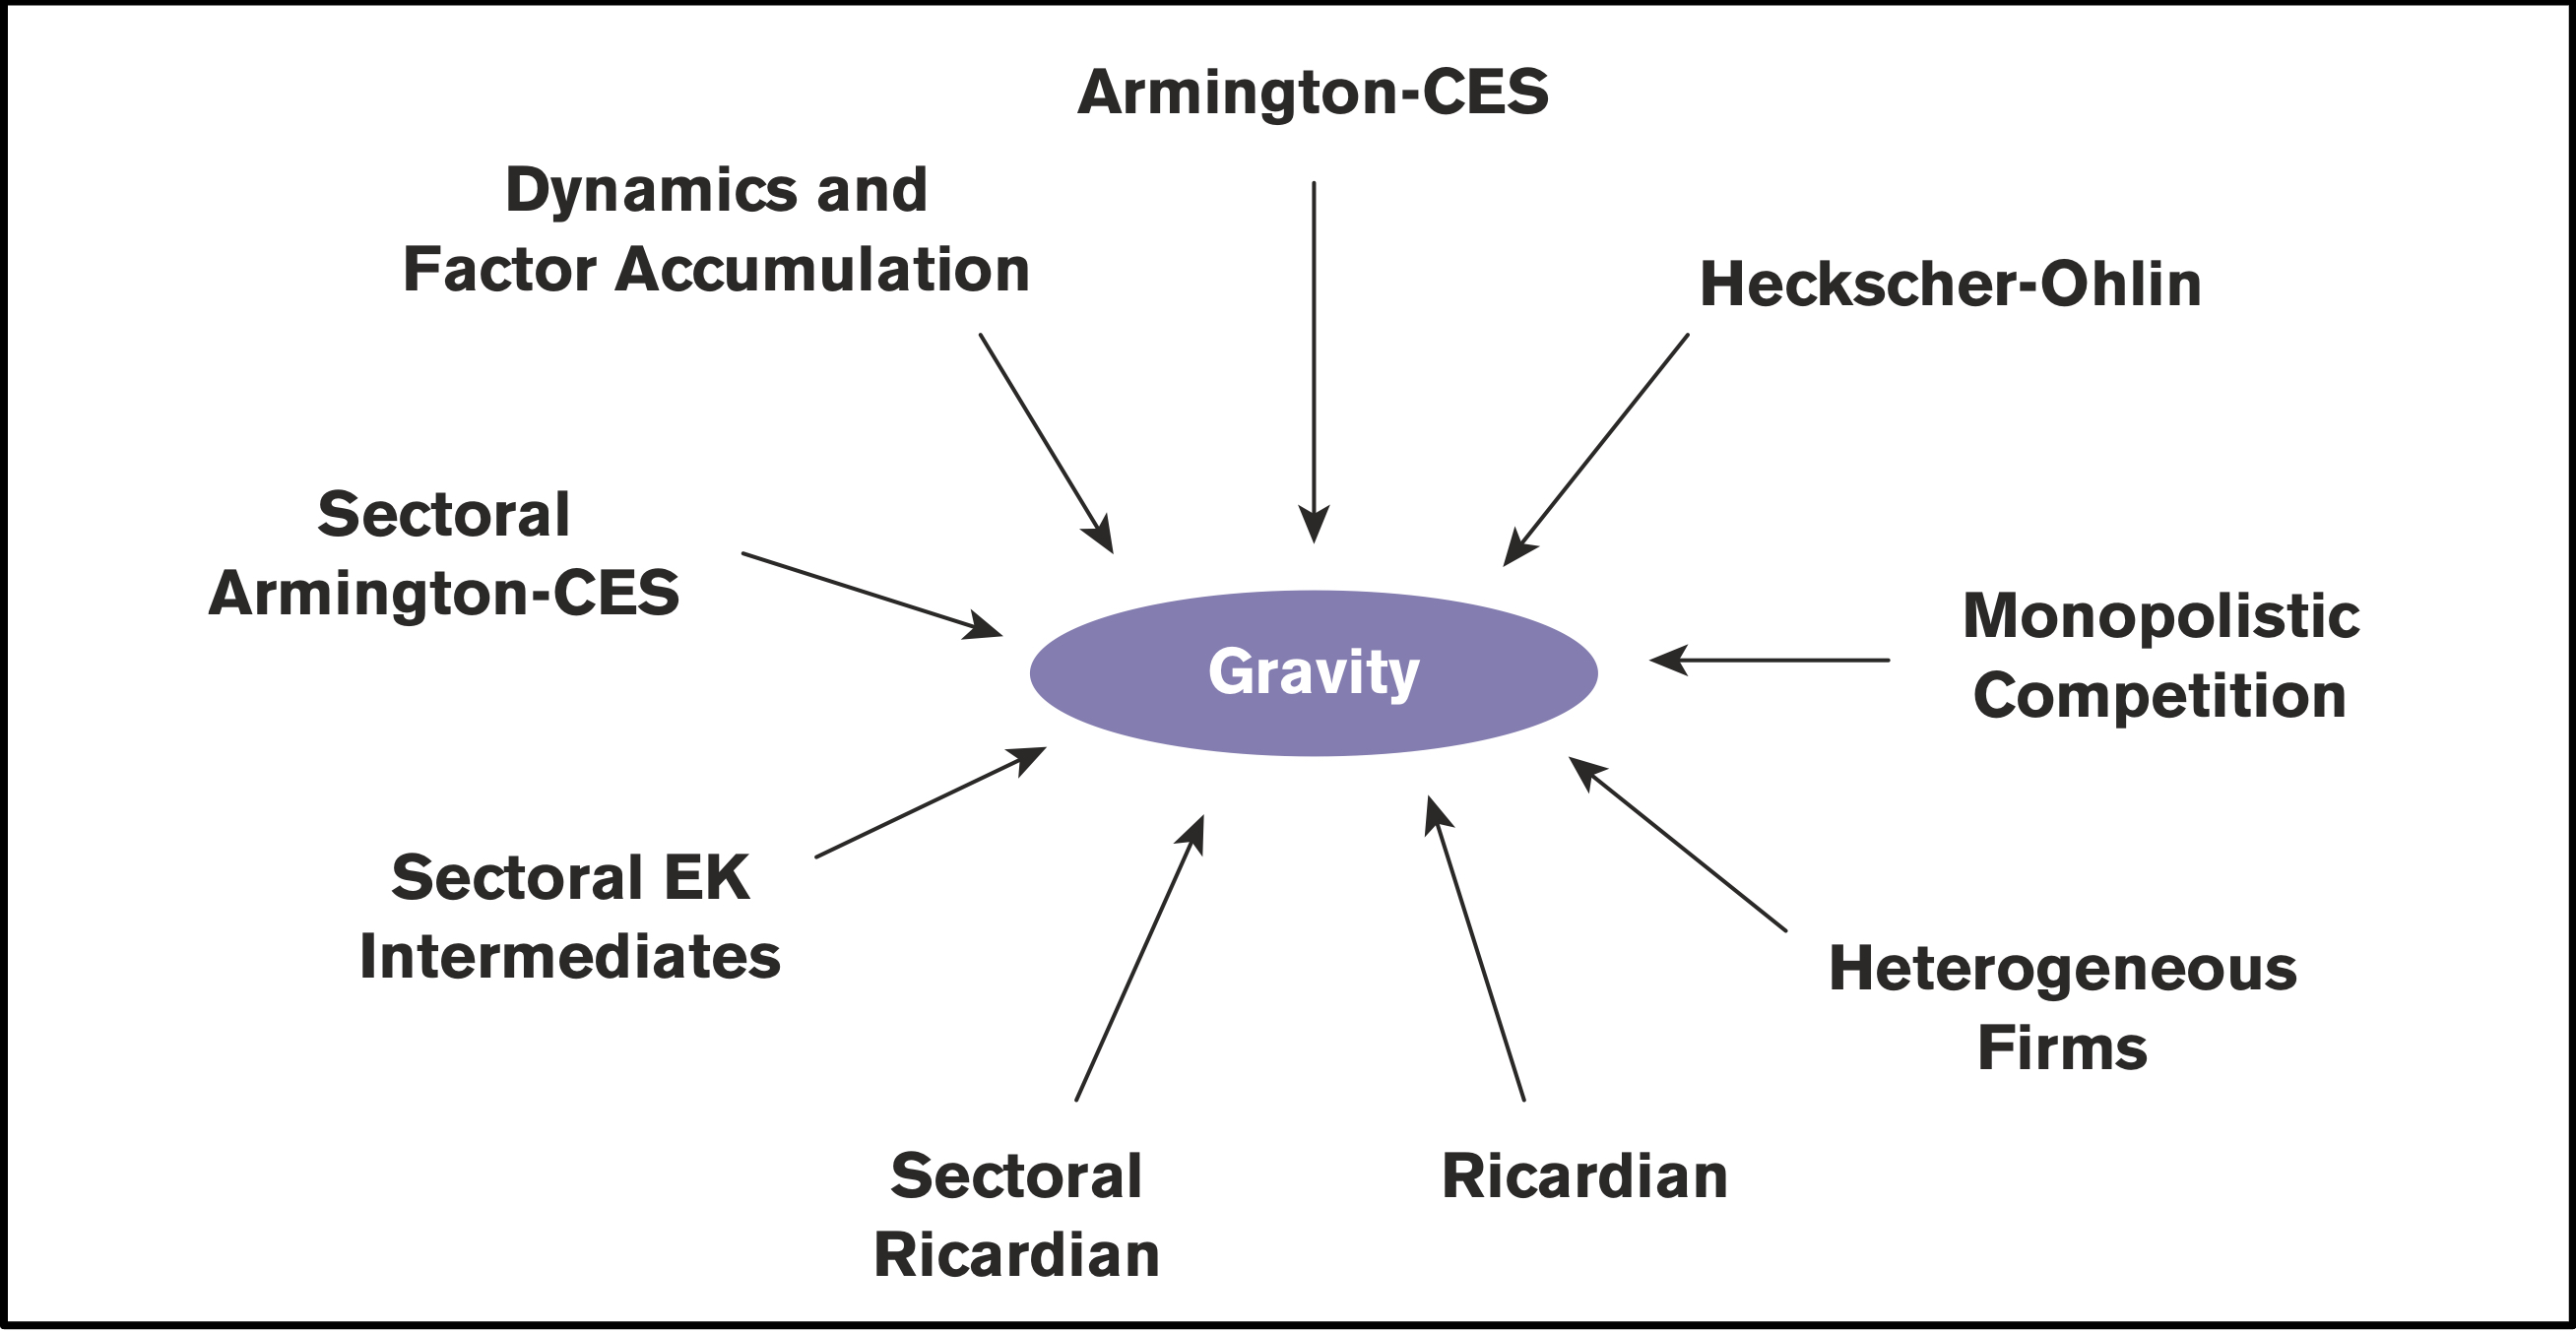
\includegraphics[width=1\textwidth]{IFME/Graphs/foundations.jpeg}
    \label{fig:theoretic_foundations}
    \small 
    Figure Source: \cite[p. 12]{yotov2016advanced}
\end{figure}

















\subsection[Estimation Tools and Challenges]{Estimation Tools and Challenges$^{\text{ JE}}$}
\label{subsec:estimation_tools}


Conveniently, gravity models can generate \textit{isomorphic} equations (\cite[p. 13]{yotov2016advanced}). This property means that the form of the trade gravity equation can be generalized or adapted to fit different contexts or additional relevant variables, maintaining its core structural properties. For instance, the simple gravity model can easily be prolonged by a vector of additional explanatory variables or elasticity parameters, like distance or cost elasticities. When it comes to equation \ref{eq:Structural_Model_LIN}, $t_{ij,t}$, $P_{j,t}$ and $\Pi_{i,t}$ are not directly observable in data. So there is a need for proxies that capture the implied trade costs and multilateral resistance terms sufficiently.   

Before \textcite{Anderson2003} highlighted the importance of multilateral resistance terms, the gravity trade model mainly had a bilateral setup. Identifying bilateral costs of trade therefore was (and still is) one of the main challenges in the estimation process. The standard procedure is to include covariates that can be observed through data and estimate the log-linearized equation \ref{eq:Structural_Model_LIN} using the ordinary least squares (OLS) estimator. \textcite[p. 21]{yotov2016advanced} list the following covariates as the most often incorporated ones: \begin{equation}
    \label{eq:bil_trade_costs_SGE}
    (1-\sigma) \ln{t_{ij,t}} = \beta_1 \ln{\underbrace{\text{DIST}_{ij}}_{\underset{\text{distance}}{\text{spatial}}}} + \beta_2 \underbrace{\text{CNTG}_{ij}}_{\underset{\text{dummy}}{\text{border}}} + \beta_3 \underbrace{\text{LANG}_{ij}}_{\underset{\text{dummy}}{\text{language}}} + \beta_4 \underbrace{\text{CLNY}_{ij}}_{\underset{\text{dummy}}{\text{colonial-ties}}} + \beta_5 \underbrace{\text{RTA}_{ij,t}}_{\underset{\text{dummy}}{\text{RTA}}} + \beta_6 \underbrace{\Tilde{\tau}_{ij,t}}_{\ln{(1+\text{tariff}_{ij,t})}}
\end{equation} Section \ref{sec:Determinants_of_Trade} will present further specifications of the bilateral trade costs. Note however that tariffs imposed by economy $j$ on exports from $i$ to $j$ at time $t$ enter the regression as $\ln{(1+\text{tariff}_{ij,t})}$ to avoid loosing observations in which there is no tariff.\footnote{There is no number $x$ such that $e^x=0$, so these observations would be dropped in an OLS regression.} This is important, since the trade elasticity of substitution ($\sigma$) is one of the main interests of researchers constructing gravity analysis and it can be approximated by the coefficient $\beta_6$ due to the fact that tariffs are direct price shifters of the traded goods and services (\cite[p. 21]{yotov2016advanced}).


The transition from only using a bilateral gravity setup to modeling a multilateral gravity equation also becomes a challenge when performing empirical estimation. \textcite{NBERw12516} introduce the term \textit{Gold Medal Mistake} as an expression for simply neglecting the multilateral resistance introduced by \textcite{Anderson2003}. $P_{j,t}$ and $\Pi_{i,t}$ from equation \ref{eq:Structural_Model_LIN} are not observed data but rather constructed in the derivation of the structural gravity model. However, not including any measures for these terms should bias the results, since their theoretical foundations of a multilateral system is still important for the gravity model. \textcite{Anderson2003} use a specific form of \textit{iterative custom nonlinear least squares programming}\footnote{The intuition is that the model is iteratively estimated over and over again with a flexible set of resistance terms until convergence, so the results do not change anymore (\cite[p. 18]{yotov2016advanced}).} to construct a set of multilateral resistances. A simpler approach would be to include so called \textit{remoteness indices} in the estimation. These indices are usually constructed in a way to capture bilateral distance and economic masses relative to world mass (expressed as GDP). \textcite{Kimura2006} for example use such a remoteness index to apply the gravity equation to trade in services.\footnote{Implications of \textcite{Kimura2006} will be discussed in later sections.} As indices constructed like that only proxy remoteness in a broad way and not fully resemble the theoretical idea of a multilateral trade system, more recent literature marks the their inclusion as insufficient to capture multilateral resistance. \textcite[p. 150]{cookbook} illustrate the issue like this: \begin{equation}
    \label{eq:REM1}
    \text{REM1}_n = \sum_i \left(\frac{\text{Dist}_{ni}}{Y_i}\right)
\end{equation} \begin{equation}
    \label{eq:REM2}
    \text{REM2}_n = \left(\sum_i \left(\frac{Y_i}{\text{Dist}_{ni}}\right)\right)^{-1}
\end{equation} In the remoteness index presented in equation \ref{eq:REM1}, very small countries are disproportionately accounted for, as $Y_i$ (GDP) is very small for them. The $\text{REM2}_n$ measure from equation \ref{eq:REM2} fixes this problem to some extend in the way that a very small $Y_i$ leads to lower effects when entering the regression as explanatory variable, as does a high $Dist_{ni}$. However, it is still not consistent with the underlying theory of remoteness factors in the way that the multilateral trade system is not represented properly (\cite[p. 151]{cookbook}). Additional alternatives to handle multilateral resistance terms would be (i) to drop them ($P_{j,t}$ and $\Pi_{i,t}$) out of equation \ref{eq:Structural_Model_LIN} by applying suitable ratios derived from equation \ref{eq:Structural_Model_NF}, (ii) to employ a dual version of the gravity model that uses techniques from spatial econometrics to include interdependence between trade flows of two economies and events happening in the rest of the world as suggested by \textcite{dualapproach}\footnote{This approach is well suited for cross-sectional data but is difficult to translate into a multi-period setup with panel data.}, or (iii) to use directional (exporter and importer) fixed effects for a cross-sectional data setup and directional time- and group-fixed effects for longitudinal data, respectively (\cite[p. 18-19]{yotov2016advanced}). One advantage of the fixed effects approach is that they will also control for other unobservables that vary over countries (policies etc.) or over time (outside shocks etc.).\footnote{\textcite[p. 152]{cookbook} even state that the inclusion of fixed effects can control for overstatements in data. They give the example of Belgium's port in Antwerp or Netherlands's port in Rotterdam to illustrate that a large amount of exports and imports flow through these stations. While the relevant trade data should only represent the commodities' origin country of production, used warehouses and reporting errors could lead to an overstatement of the port-countries exports (or imports). Such data discrepancies can also be absorbed by fixed effects (\cite[p. 152]{cookbook}). Note that this issue relates mainly to trade in goods, while for trade in services other problems arise (see section \ref{sec:Service_Models}).} Another pro-argument for the inclusion of fixed effects is that they can help to mitigate the estimation bias induced by potential (and likely) endogeneity of trade policies like RTAs. Such trade policies obviously are an important covariate when explaining trade patterns and determining the costs of trade. The decision to engage in contracts of lowering trade barriers is, however, also likely to be correlated to other explanatory variables (like distance or language barriers) and therefore brings up the issue of endogeneity (\cite[p. 21]{yotov2016advanced}). Finding and assessing relevant and exogenous instrumental variables is an ongoing struggle in the literature, especially for applications to international trade. That is why combining different econometric approaches with fixed effects and multiple robustness checks can be described as the go-to approach to address potential endogeneity of trade policies (\cite{trade_agreements_2024}, \cite[p. 21]{yotov2016advanced}).

While having the above mentioned advantages, the inclusion of fixed effects can also lead to problems in consistent estimations of gravity models, as they might absorb impacts that other covariates have on trade which are subject to the analysis. One prominent example are non-discriminatory trade policies\footnote{Non-discriminatory trade policies require that countries treat trading partners equally, offering the same terms to all under the \textit{most-favoured-nation} principle, and that imported goods receive the same treatment as domestic products, known as \textit{national treatment}. These principles aim to ensure fairness and prevent biases in international trade practices but can also be dominated by special forms of market integration like RTAs (\cite{wto_nondiscrimination}).} (\cite[p. 22]{yotov2016advanced}). The intuition is that if such policies are in place, the analyst is interested in their effects. However, as they are non-discriminatory, they can be viewed as a country fixed effect and their impact is not accounted for, if fixed effects are included (\cite{heid2015simple}). Besides the less theory founded method of including remoteness indices or a two-stage estimation process where non-discriminatory trade policies are included in the first stage, \textcite{heid2015simple} propose to adjust the gravity framework by also including \textit{intranational} trade data. Policies that are non-discriminatory are assumed to not effect domestic trade and thus, the inclusion of such data can help to recover the estimates of policies like \textit{most-favoured-nation} (MFN) tariffs in a properly adjusted framework (\cite{heid2015simple}).

Another problem arising with specifications that include fixed effects (in the \textit{normal way}) is that adjustments to trade policies take time until the effects show up in data and this time lag of reaction is not accounted for. \textcite[p. 23]{yotov2016advanced} summarize the literature's response to that issue in the finding that using pooled intervals when dealing with longitudinal data helps to control for time lags and results in more precise trade cost elasticity estimates.

A further challenge to overcome is sectoral heterogeneity. Since different sectors might be described by strongly differing characteristics, such as trade costs or competition levels, a more disaggregated view on the gravity model might be needed (\cite[p. 23]{yotov2016advanced}). This argument is important for the discussion of differences in trade in goods and trade in services as well as differences inside different good sectors and inside service sectors. Depending on the data and application at hand, a more disaggregated view can be generated by allowing directional fixed effects and policy effects to differ across sectors (\cite[p. 23]{yotov2016advanced}).

To conclude the short review and discussion about challenges and tools in the estimation process of gravity equations, two more important points have to be brought up. First, the literature is well aware that data on international trade is usually subject to heteroscedasticity\footnote{Heteroscedasticity refers to a situation in which the variance of the residuals differs along the conditional distribution of an independent covariate (\cite[p. 190]{stock2019}). A log-linearized OLS estimation then would produce biased coefficients.} (\cite{trade_agreements_2024}, \cite{Greaney2020}, \cite{KABIR201760}, \cite[p. 23]{yotov2016advanced}). Secondly, if the trade data contain flows of zero, this also holds valuable information for the implied effects of other covariates, especially in the case of highly disaggregated data. However, in a setting in which the OLS estimator is applied to equation \ref{eq:Structural_Model_LIN}, all those observation would be omitted in the estimation process due to the above mentioned fact that the log of zero is not defined.\footnote{Due to intensively localized consumption and specialized production, this is a standard cause of bias especially when applying gravity analysis to trade in services (\cite[p. 19]{yotov2016advanced}).} Both these challenges can be overcome by using the Poisson Pseudo Maximum Likelihood (PPML) estimator (\cite[p. 20]{yotov2016advanced}).\footnote{Examining the PPML estimator would go beyond this seminar paper. The estimation technique can be traced back to \textcite{Pseudo_M_likeli}. It is a widely used tool which was subject to Monte Carlo simulations and was found to handle zero trade flows as well as heteroscedastic data quit well and is therefore prominently used in gravity applications (\cite{trade_agreements_2024}).} There have also been other methods proposed to handle the zero trade flow issue. One straightforward approach is to add a very small number to trade flows before logging them. However, this can distort coefficient interpretations as elasticities, since measurement units matter (\cite[p. 21]{yotov2016advanced}). Another theoretically grounded approach is the Helpman, Melitz, and Rubinstein (HMR) model (\cite{HelpmanElhanan2008ETFT}), which uses a two-step selection process. The first stage estimates the probability of trade, using a probit (or logit) model, followed by OLS estimation on a sample that is adjusted by these first stage probabilities. Yet, this method's reliance on functional form in combination with the difficulty of finding valid exclusion restrictions pose significant challenges, especially in longitudinal data settings (\cite[p.19]{yotov2016advanced}). An alternative is the two-part gravity model by \textcite{EGGER2011263}, which decomposes the explanatory variables' effects into extensive (decision to export) and intensive (volume of exports) margins. This model also addresses biases from endogenous regressors and improves estimation accuracy (\cite[p. 19]{yotov2016advanced}).

The different tools and estimation methods reviewed above should be kept in mind when interpreting results and implications of gravity models for both trade in goods and services.










































































